\chapter{Introduction}

There is an increasing awareness of the potential benefits of intelligent energy control of the balance between the distributed energy resources and the demand requirements. Intelligent energy control leads to efficient planning, more satisfied consumers and can even help National Electricity Markets in saving considerable operating and maintenance cost according to \cite{NarjesFallah2018}. Having accurate forecasting models is one of the key conditions to in practise realize intelligent energy control. When electricity consumption forecasting is improved, energy producers can build a better trust with its customers by sending reliable bills. Further, can the electricity producer better estimate the energy demand of the whole customer population. The optimization of the energy production planning is possible, which will lead to cheaper electricity production and increased profit margins. More substantiated decisions can be taken with regard to investments and there will be less need of the more flexible but more expensive electricity installations e.g. diesel engines to catch the deficiencies in electricity production.\\

With the invention of the smart meter in 1977 by \textbf{Paraskevakos} it became possible to communicate the electricity consumption with more clarity to the consumer and the electricity producer. Electricity consumption is nearly recorded real time and it allows for two-way communication between the smart meter and the supplier. As explained in \cite{Depuru2011}: ``By introducing smart meters as a new
component of their smart grid system, an avalanche of immensely useful energy usage information
became available to the energy markets.'' From the availability of more detailed datasets flows the explosion of research in the electrical forecasting techniques and the applicability of more complex models. To tackle the 

Also machine learning tools and neural networks

The reason for the explosion in 


Congestion forecasting during network changes





When forecasting is improved on household scale, the customer can be better informed what the bill is going to be at the end of the month/year.
Energy producer can build a better trust with its customer by sending reliable bills. (Providing good service)
Producent can better estimate the energy demand of the whole customer population. This will lead to cheaper electricity production because a better planning is possible where there is less need of the more 
flexible but more expensive electricity installations e.g. diesel engines.



Having reliable forecasts available will play a decisive role in the exploitation of 


 Accurate and reliable forecasting techniques   




\begin{figure}[hb]
	\centering
	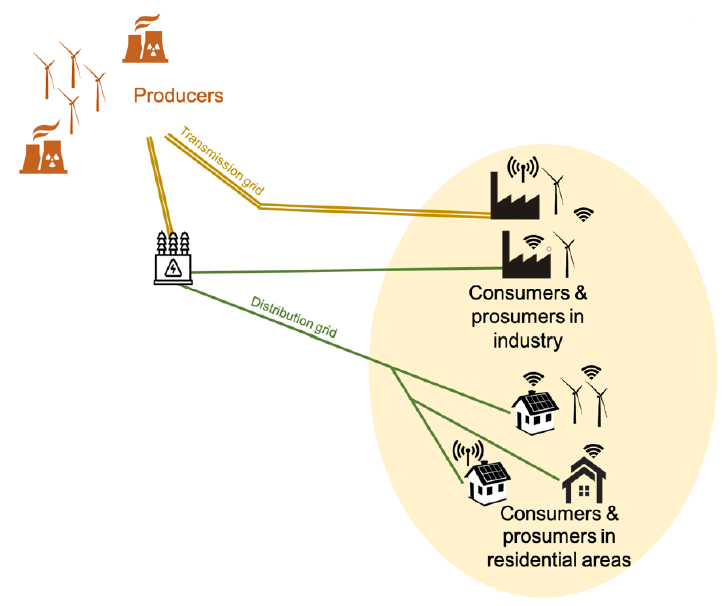
\includegraphics[width=1.0\textwidth]{SmartGrid.png}
	\caption{Electricity grid (Source: KU Leuven thesis proposal).}
	\label{fig:power_image}
\end{figure}


- different kinds of loads

- different often used metrics. 

- make the transition to short term and why this is important. 


\section{Importance of topic}
Individual household forecasting is a complex task because of the high amount of uncertainty
and the volatility of the data. To deal with this it was found in literature that often aggregated signals are forecasted instead. If there are papers that discuss electrical household consumption forecasting, they often use a lot of information about the household which will not be scalable in practice due to privacy concerns. This thesis investigates state of the art time series forecasting techniques based on LSTM neural networks that have as goal to forecast the next day of electrical household consumption, given only limited information.\\

When forecasting is improved on household scale, the customer can be better informed what the bill is going to be at the end of the month/year.
Energy producer can build a better trust with its customer by sending reliable bills. (Providing good service)
Producent can better estimate the energy demand of the whole customer population. This will lead to cheaper electricity production because a better planning is possible where there is less need of the more 
flexible but more expensive electricity installations e.g. diesel engines.

- Like in pooling paper --> talk about methods that are used to reduce complexity/ already written in --> now directly forecasting the individual household consumption --> very complex task. 


- see also table PL. 

- working with real-life data

- wie zijn mijn assessoren? 

- local prediction can be important for local changes to the net --> see oneNote goal PL.

- look at goal of thesis --> meeting and PL goal --> what do they want to do exactly

The weather and calendar data is correlated with the energy load profiles

\section{Problem formulation and link with previous studies}
Now going to forecast individual houses, not aggregated signals. 

Things were I should get familiar with: scikit-learn, Tensorflow, Keras, Pandas, Anaconda, Microsoft Azure --> step in improving software skills.

Not just looking at regular data --> individual household data --> not a day will be the same and only have limited information available. These two together makes the forecasting extremely difficult. 


\section{Thesis objective and structure}
The goal of this thesis is to do short-term load forecasting for individual households. A forecast of the electrical load of a household for 24 hours. 

Develop a model for the future prediction of smart meter electric power consumption. The final
objective is to compare several existing methods

%%% Local Variables: 
%%% mode: latex
%%% TeX-master: "thesis"
%%% End: 
